\documentclass[12pt]{article}

\usepackage[utf8]{inputenc}
\usepackage{geometry}

\usepackage{hyperref}
\usepackage{fancyhdr}

\usepackage{graphicx}
\usepackage{float}

\usepackage{listings}
\usepackage{color}

\usepackage[T1]{fontenc}


\setlength{\headheight}{15pt}
\pagestyle{fancy}
\fancyhf{}
\rhead{Computer Workshop Course}
\lhead{Final Assignment}
\rfoot{Page \thepage}


\definecolor{dkgreen}{rgb}{0,0.6,0}
\definecolor{gray}{rgb}{0.5,0.5,0.5}
\definecolor{mauve}{rgb}{0.58,0,0.82}

\lstset{frame=tb,
	language={},
	aboveskip=3mm,
	belowskip=3mm,
	showstringspaces=false,
	columns=flexible,
	basicstyle={\small\ttfamily},
	numberstyle=\tiny\color{gray},
	keywordstyle=\color{blue},
	commentstyle=\color{dkgreen},
	stringstyle=\color{mauve},
	breaklines=true,
	breakatwhitespace=true,
	tabsize=4,
	numbers=left,
	stepnumber=1
}



\title{Computer Workshop \\ Final Assignment}
\author{Ali Mozdianfard}
\date{January 2024}



\begin{document}
	
	\begin{titlepage}
	    \maketitle
	    \thispagestyle{empty}
	\end{titlepage}

	\newpage

	\tableofcontents
	\newpage
	
	\section{Git \& GitHub}
	Here is every step of the process of creating the repository of this assignment
	and setting up the GitHub Actions for compiling \LaTeX.
	
	\begin{figure}[H]
		\centering
		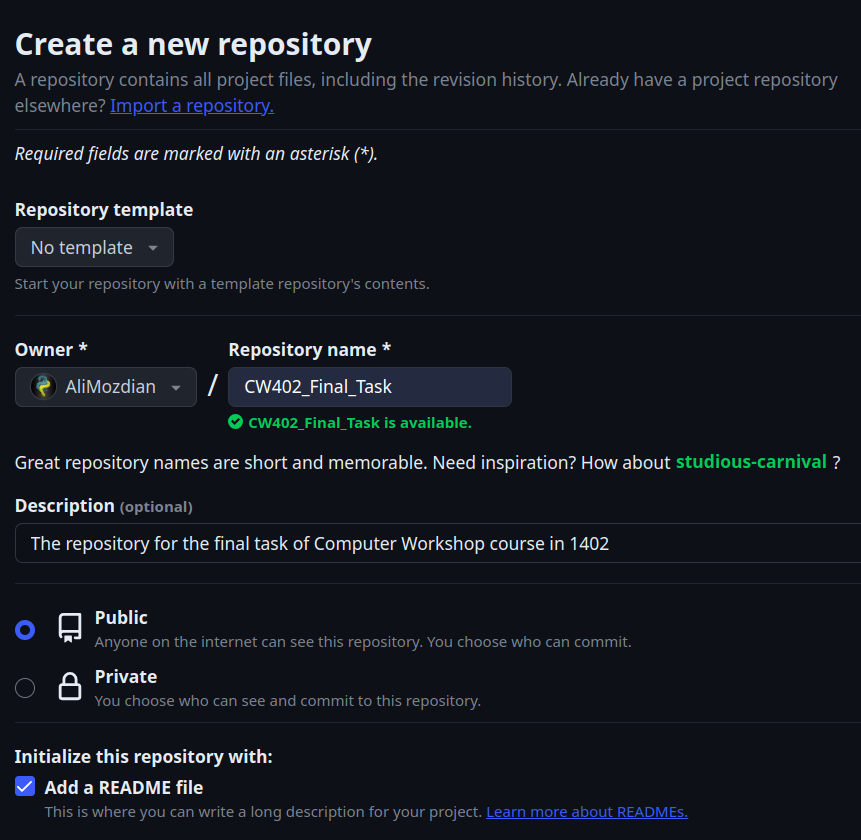
\includegraphics[width=\textwidth]{images/ss0.png}
		\caption{Creating the repository in GitHub}
	\end{figure}
	
	\begin{figure}[H]
		\centering
		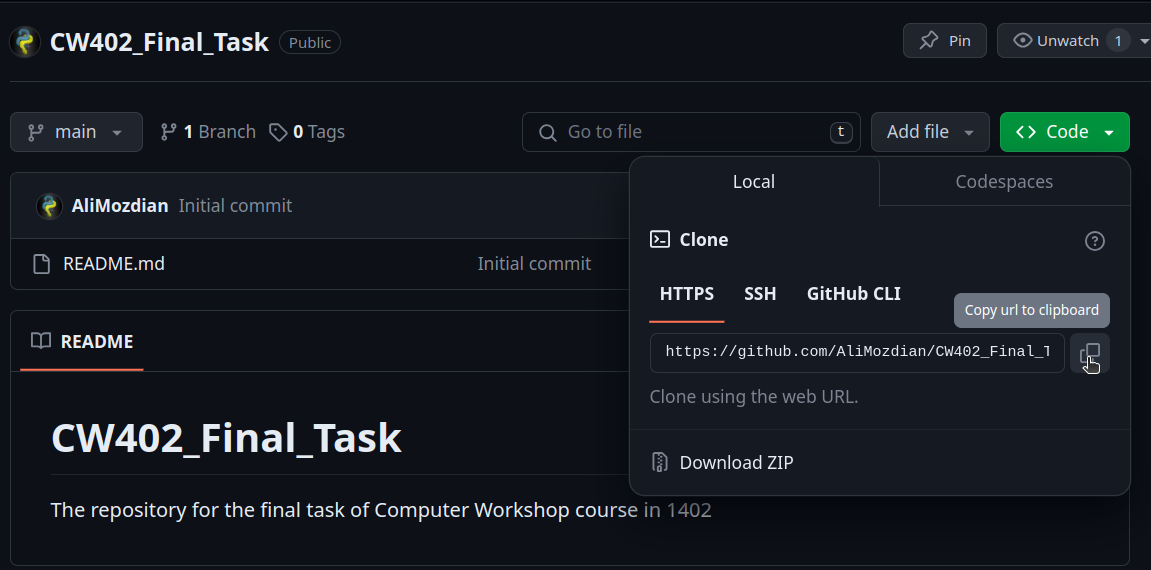
\includegraphics[width=\textwidth]{images/ss1.png}
		\caption{Copying the link of HTTPS link for cloning the repository into my local machine}
	\end{figure}
	
	\begin{figure}[H]
		\centering
		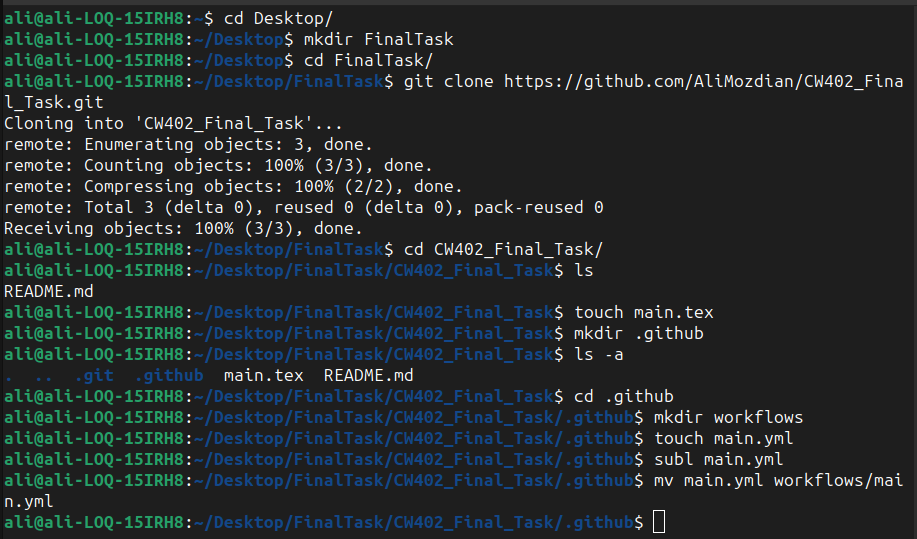
\includegraphics[width=\textwidth]{images/ss2.png}
		\caption{From now on we will be doing the needed setup for GitHub Actions. \\ Creating the needed files for the project.}
	\end{figure}
	
	\begin{figure}[H]
		\centering
		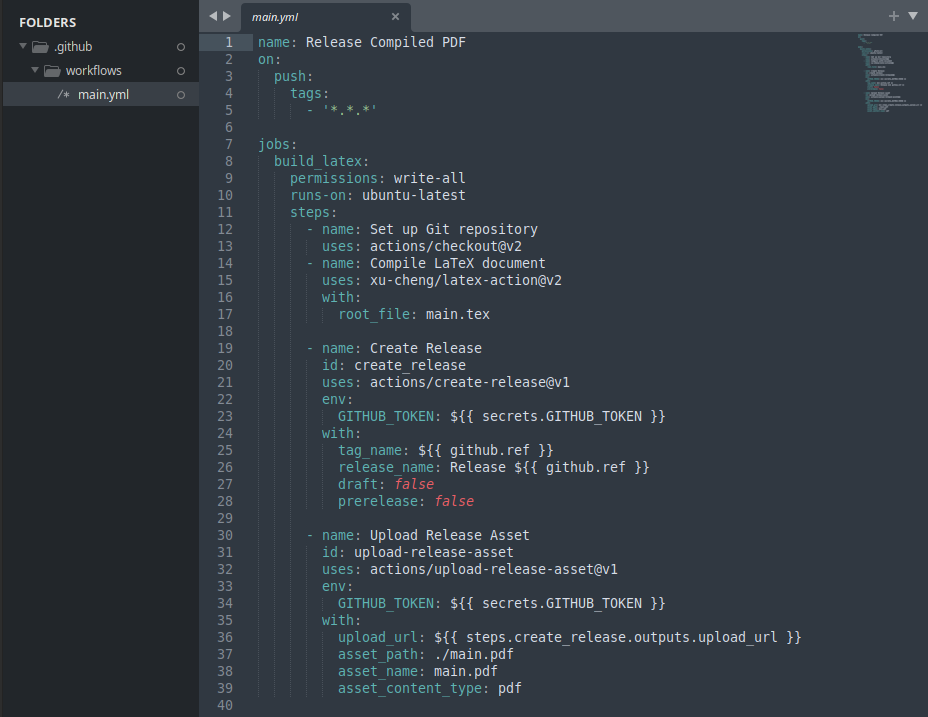
\includegraphics[width=\textwidth]{images/ss3.png}
		\caption{Writing in main.yml to set GitHub Actions (.github/workflows/main.yml)}
	\end{figure}
	
	\begin{figure}[H]
		\centering
		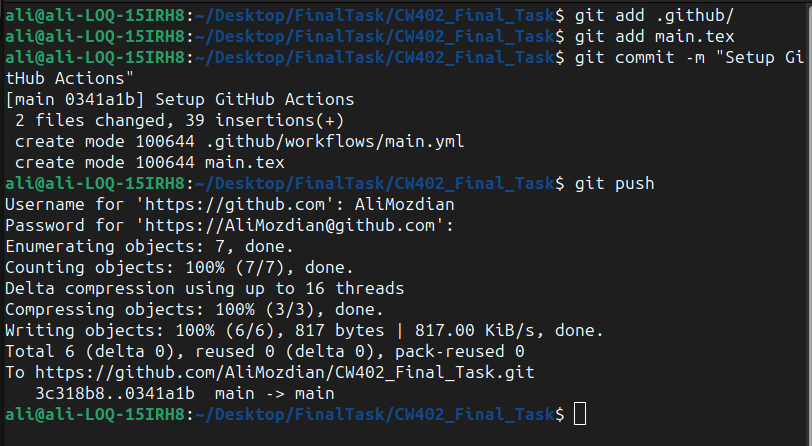
\includegraphics[width=\textwidth]{images/ss4.png}
		\caption{add, commit and push, then we are ready to start the project, but tags!}
	\end{figure}
	
	\begin{figure}[H]
		\centering
		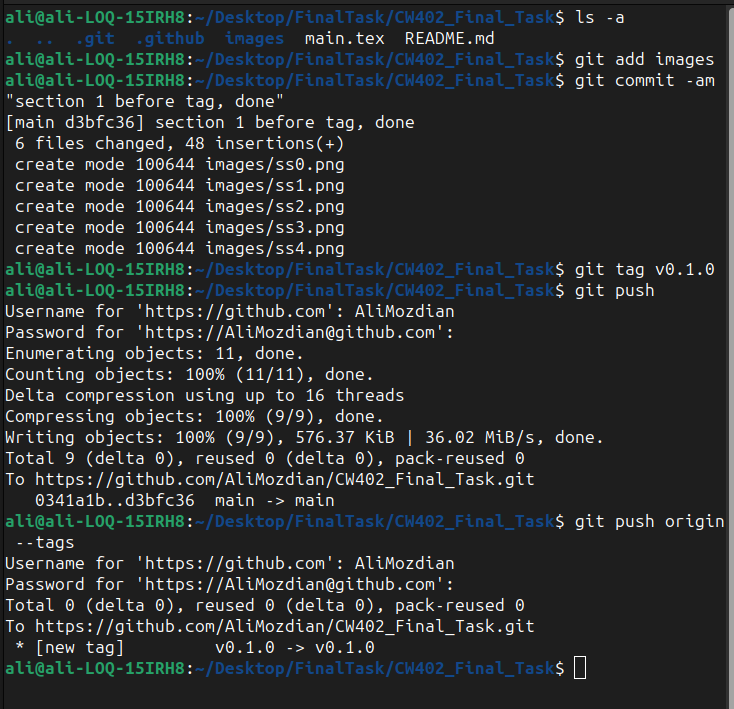
\includegraphics[width=\textwidth]{images/ss5.png}
		\caption{Adding and commiting the images, also making a tag for this commit. \\ then pushing the repo and its tags (via two commands)}
	\end{figure}
	
	\begin{figure}[H]
		\centering
		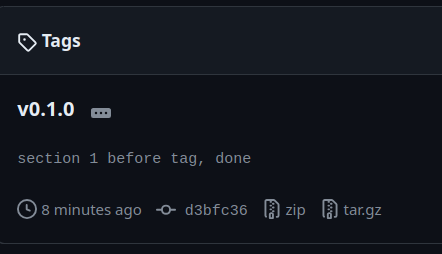
\includegraphics[width=\textwidth]{images/ss6.png}
		\caption{As you can see the tags now are in GitHub as well}
	\end{figure}
	
	\begin{figure}[H]
		\centering
		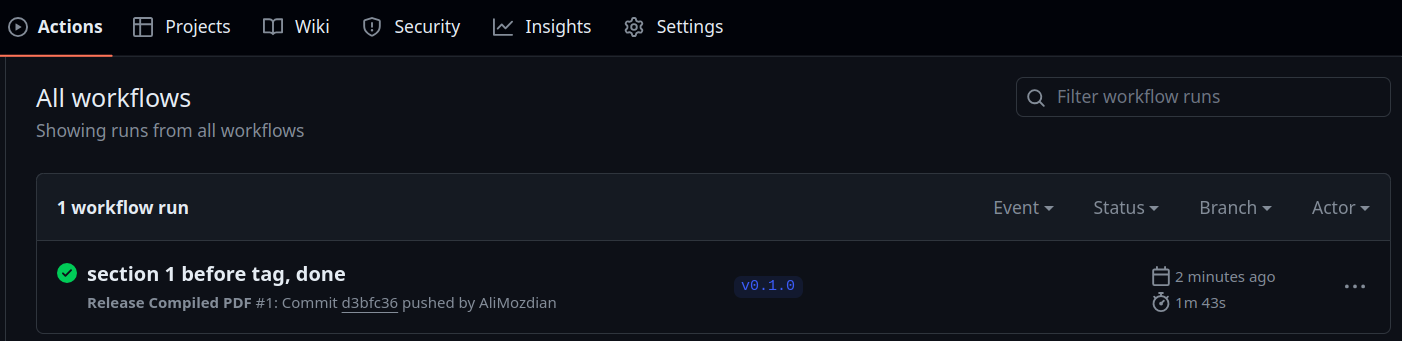
\includegraphics[width=\textwidth]{images/ss7.png}
		\caption{And becuase of the format of the tag, GitHub Actions complied it without a problem}
	\end{figure}
	
	So just repeat this cycle:
	\begin{enumerate}
		\item make changes
		\item git add
		\item git commit
		\item git tag
		\item git push
		\item git push tags
		\item GitHub Actions compiles the main.tex automatically
	\end{enumerate}

	\section{Exploration Tasks}
	\subsection{Vim Advanced Features}
	In this section we are going to learn about three advanced features of VIM that you might doesn't expect them:
	\begin{enumerate}
		\item Multiple Windows and Tabs
		\item Folding
		\item Scripting
	\end{enumerate}

	Here I've search about them and made a short document for each of these 3 above.

	\subsubsection{Multiple Windows and Tabs}
	\paragraph{Multiple Windows:} In Vim, windows refer to individual panes within the editor's interface, each displaying a different section of the same or different file.
	By splitting the editing window into multiple windows, users can view and edit different parts of a file concurrently, facilitating seamless multitasking and improving workflow efficiency.

	Some of the key commands to do so:
	\begin{itemize}
		\item ":vsp" $\rightarrow$ splits window vertically (or you can use ":vertical split")
		\item ":sp" $\rightarrow$ splits window horizontally (or you can use ":split")
		\item "Ctrl + w" $\rightarrow$ navigate between windows (use it followed by arrow keys to do it more efficiently)
		\item "Ctrl + w" followed by '$>$' or '$<$'' $\rightarrow$ to increase or decrease window size.
	\end{itemize}

	\paragraph{Tabs:} Vim also supports the use of tabs, allowing users to work with multiple files within the same Vim session.
	Each tab represents a separate editing session, with its own set of windows and buffers, providing a convenient way to organize and
	switch between different files or projects.

	Some of the key commands to do so:
	\begin{itemize}
		\item ":tabnew" or ":tabnew $<$filename$>$" $\rightarrow$ opens new tab
		\item "gt" $\rightarrow$ switch to the next tab
		\item "gT" $\rightarrow$ switch to the previous tab
		\item ":tabclose" $\rightarrow$ close tab
	\end{itemize}

	\subsubsection{Folding}
	Folding in Vim is a feature that allows you to collapse or "fold" sections of text within a file, making it easier to focus on specific parts of the document while hiding others.
	It's particularly useful for navigating large files, organizing code, and managing complex structures such as functions, classes, or sections of documentation.
	In general, there is two types of folding in VIM, Manual Folding and indentation-based Folding.

	Some of the key commands to do so:
	\begin{itemize}
		\item zf followed by a motion $\rightarrow$ create a fold for the text covered by the specified motion.
		\item za $\rightarrow$ toggle fold and unfold at the position that cursor points at.
		\item zd $\rightarrow$ delete the fold at the cursor without deleting its contents, just the fold itself.
	\end{itemize}

	\subsubsection{Scripting}
	Vimscript is a powerful scripting language built into Vim, allowing users to automate tasks and customize Vim's behavior extensively.
	Vimscript functions can be defined to perform specific actions, and custom commands can be created to execute sequences of Vim commands conveniently
	Example of defining a Vimscript function to perform a custom action:

	\begin{lstlisting}
	function! MyCustomFunction()
    	" Vimscript code goes here
		endfunction
	\end{lstlisting}

	Example of creating a custom command to execute the above function:

	\begin{lstlisting}
	command! MyCommand call MyCustomFunction()
	\end{lstlisting}


	With custom commands and functions, users can automate repetitive tasks, create complex editing workflows, and enhance Vim's functionality to suit their specific needs.

	\subsection{Memory Profiling}
	\subsubsection{Memory Leak}
	Memory leaks occur when a program allocates memory dynamically but fails to release it properly when it's no longer needed.
	As a result, memory that is no longer in use remains allocated, leading to wastage of system resources.
	Over time, repeated memory leaks can deplete available memory, causing the program or even the entire system to slow down or crash.
	
	Causes of Memory Leaks:
	\begin{itemize}
		\item failure to free memory: For example not use free function in C, after you're done using malloc.

		\item lost refrences: Losing track of pointers or references to dynamically allocated memory blocks can prevent the program from releasing them

		\item cyclic refrences: In languages with automatic garbage collection (like java), cyclic refrences between two or more objects can prevent them from being garbage collected.

		\item unclosed resources: Not closing the opened resources after you're done using them, like file handles, network connections, etc.
	\end{itemize}

	\subsubsection{Memory Profilers}
	\paragraph{Valgrind} is an open-source tool designed for debugging and profiling programs on Unix-like operating systems and it is a powerful tool for detecting and preventing memory leaks and other memory-related issues in software programs.
	By providing detailed analysis and insights into memory usage and behavior, Valgrind helps developers identify and fix memory-related problems early in the development process, resulting in more reliable and efficient software systems.
	Also one of the most widely used Valgrind tools for memory debugging is called Memcheck.

	But the question remains that how does Valgrind helps with preventing memory leaks? We shortly discuss about it here.

	\begin{itemize}

		\item Memory Leak Detection:
		Valgrind's Memcheck tool can detect memory leaks by tracking dynamically allocated memory blocks throughout the program's execution.
		It identifies memory blocks that have been allocated but not deallocated, providing detailed information about their allocation point in the code.
		This helps developers identify memory leaks and understand the root causes, facilitating timely fixes.

		\item Memory Access Errors:
		Valgrind can also identify various memory access errors, such as reading from or writing to uninitialized memory, accessing freed memory, and buffer overflows. Detaching these errors early in the development process, can lead to preventing potential memory corruption issues, which is very important to prevent these issue from the begining of their hidden existance.

	\end{itemize}

	There are many of them (these methodes) but I think it suffices to say how usefull and important is this concept in programming, and it is the answer to why should we give credit to the tools which prevent this.


	\subsection{GNU/Linux Bash Scripting}
	\subsubsection{fzf}
	\paragraph{What is fuzzy searching?}
	Fuzzy searching, as used in tools like fzf, is a technique that allows for approximate matching of search patterns. Instead of requiring an exact match.
	Fuzzy searching considers variations in spelling, word order, and character sequences to find relevant results, enhancing search flexibility and efficiency.

	\paragraph{What does "ls | fzf" does?}
	The pipe character ('|') means that give the output of "ls" as the input of "fzf".
	"ls" command lists files and directories in the current directory
	and "fzf" uses fuzzy searching, so combinded with eachother,
	it provides an interactive way to search and select files and directories from the current directory using fuzzy matching, enhancing navigation within the terminal.

	\subsubsection{Using fzf to find you favorite PDF}
	Because of shortage of time, in this part, I just type the answers:
	\begin{itemize}
		
		\item fd -e PDF

		\item fd -e PDF | fzf

	\end{itemize}

	\subsubsection{Opening the file using Zathura}
	zathura "\$(fd -e PDF | fzf)"


	\section{Git and FOSS}
	
	\subsection{Issues}

	\begin{figure}[H]
		\centering
		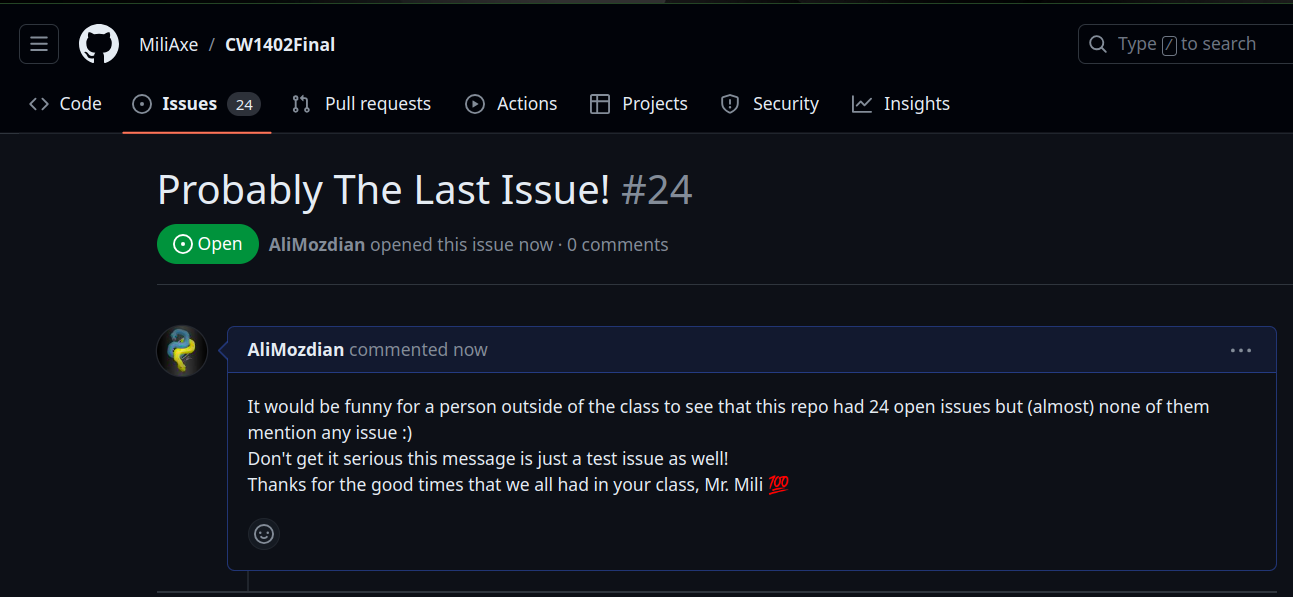
\includegraphics[width=\textwidth]{images/ss8.png}
		\caption{The asked screenshot of a sample issue on the mentioned repository}
	\end{figure}
	


\end{document}
